\documentclass[a4paper, 12pt]{article}%тип документа

%отступы
\usepackage[left=2cm,right=2cm,top=2cm,bottom=3cm,bindingoffset=0cm]{geometry}

%Русский язык
\usepackage[T2A]{fontenc} %кодировка
\usepackage[utf8]{inputenc} %кодировка исходного кода
\usepackage[english,russian]{babel} %локализация и переносы

%Вставка картинок
\usepackage{wrapfig}
\usepackage{graphicx}
\graphicspath{{pictures/}}
\DeclareGraphicsExtensions{.pdf,.png,.jpg}

%оглавление
\usepackage{titlesec}
\titlespacing{\chapter}{0pt}{-30pt}{12pt}
\titlespacing{\section}{\parindent}{5mm}{5mm}
\titlespacing{\subsection}{\parindent}{5mm}{5mm}
\usepackage{setspace}

%Графики
\usepackage{multirow}
\usepackage{pgfplots}
\pgfplotsset{compat=1.9}

%Математика
\usepackage{amsmath, amsfonts, amssymb, amsthm, mathtools}

%Стиль страницы
\usepackage{fancyhdr}
\pagestyle{fancy}

\begin{document}

\begin{titlepage}

\begin{center}
%\vspace*{1cm}
\large\textbf{Московский Физико-Технический Институт}\\
\large\textbf{(национальный исследовательский университет)}
\vfill
\line(1,0){430}\\[3mm]
\huge\textbf{Лабораторная работа №19}\\
\item{   }\\
\large\textbf{Задания 2, 4, 5}\\
\line(1,0){430}\\[1mm]
\vfill
\large Баканова К.В., Б01-003\\
%\vspace*{1cm}
\large апрель 2022 г.\\
\end{center}

\end{titlepage}


\section{Полосовое звено на сдвоенном усилителе.}

\newpage
\fancyhead[L] {Лабораторная работа №19}
\fancyhead[R] {Баканова К.В.}
\section{Активные звенья с двойным Т-мостом}


\begin{figure}[h!]
    \centering
    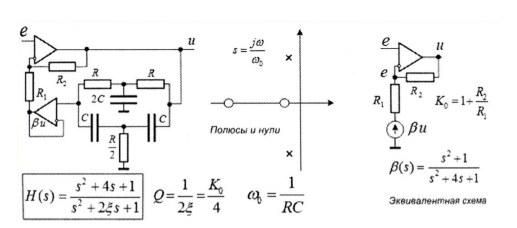
\includegraphics[width=1\linewidth]{pic5.png} 
    \caption{Полосовой фильтр с двойным Т - мостом.}
\end{figure}

\subsection{}

 Откроем модель полосового фильтра c $f_0 = 10k$, $K_0 = 20$. Измерим
усиление на частоте $f_0$ и полосу $\Delta f$ по уровню -3dB. Получаем $K_0 = 20.92$,
$\Delta f = 1.93$ ($R_2 = 20k$).


\begin{center}
\begin{tabular}{|c|c|c|c|c|}
\hline 
$R_2$, Ом & 40k & 60k & 80k & 100k \\ 
\hline 
$K_0$ & 41,02 & 61,12 & 81,11 & 101,24 \\ 
\hline 
$\Delta f$, Гц & 979 & 643 & 495 & 397 \\ 
\hline 
\end{tabular} 
\end{center}


\subsection{}

Изучим поведение фильтра при разбалансировании моста варьированием $R_5$. Снимем зависимость от $R_5$ пикового усиления.
\begin{center}
\begin{tabular}{|c|c|c|c|c|c|c|c|c|c|c|}
\hline 
$R_5$, Ом & 1,5 & 2 & 2,5 & 3 & 3,5 & 4 & 4,5 & 5 & 5,5 \\ 
\hline 
$K_0$ & 32,45 & 43,76 & 79,67 & 956,78 & 90,57 & 42,88 & 28,11 & 20,97 & 16,88 \\ 
\hline 
\end{tabular} 
\end{center}

\subsection{}
Измерим уровни скачка в нуле и первого выброса: уровень скачка - 1В при $R_5$ =
5k Ом.
Оценим значение $R_5$, при котором фильтр теряет устойчивость.

\begin{center}
\begin{tabular}{|c|c|c|c|c|c|c|c|}
\hline 
$R_5$, Ом & 5k & 4,5k & 4k & 3,5k & 3k & 2,5k \\ 
\hline 
выброс & 4,29 & 4,49 & 4,72 & 5,0 & 5,36 & 5,82 \\ 
\hline 
\end{tabular} 
\end{center}


\subsection{}

Откроем модель режекторного фильтра c $f_0 = 10k$, $\gamma = 0.1$.

\begin{figure}[h!]
    \centering
    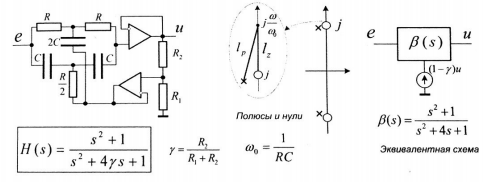
\includegraphics[width=1\linewidth]{pic9.png}
    \caption{Режекторный фильтр с двойным Т - мостом.}
\end{figure}

Измерим ширину полосы режекции $\Delta f$ по уровню 0.7 = −3dB. Получим: $\Delta f$ = 4.07 кГц.

\subsection{}


Измерим уровни скачка в нуле и первого выброса. Получим: уровень скачка - 1В, первый выброс - 697.5 мВ.

\newpage





\section{Полосовое звено на сдвоенном усилителе.}





\newpage
\fancyhead[L] {Лабораторная работа №19}
\fancyhead[R] {Баканова К.В.}
\section{Звенья Саллена-Ки.}

\begin{figure}[h!]
    \centering
    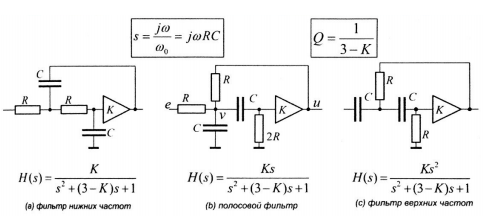
\includegraphics[width=1\linewidth]{pic10.png}
    \caption{Звенья Саллена-Ки.}
\end{figure}

\subsection{}
Откроем модель звеньев Саллена-Ки с частотой $f_0 = 10k$ и добротностью $Q = 1$.
Измерим значения коэффициентов передачи при $f = f_0$. Получим:

\begin{equation*}
    K_0 = 2, \space k_{lp} = 29.44, \space K_{hp} = 28.485, \space K_{bp} = 28.898
\end{equation*}

\subsection{}

Откроем модель с фильтрами Баттерворта верхних и нижних частот
порядка $n = 3$ на частоту среза $f_0 = 10k$. Измерим скорости спада в dB на октаву и
затухания на частотах $f_0/2$, $2f_0$:
\par
ВЧ: затухание на $f_0/2$ : −18 dB, скорость спада −15 $\frac{dB}{\text{дек}}$
дек
\par
НЧ: затухание на $2f_0$ : −18 dB, скорость спада 15 $\frac{dB}{\text{дек}}$
дек
.
\medskip
\par
Измерим уровни затухания фильтров Чебышева на частотах $f_0/2$, $2f_0$:
\par
ВЧ: затухание на $f_0/2$ : −30 dB, скорость спада −18 $\frac{db}{\text{деб}}$
дек
\par
НЧ: затухание на $2f_0$ : −30 dB, скорость спада 18 $\frac{db}{\text{деб}}$
дек
.

\subsection{}
Откроем прототип , реализуем 4-полюсной полосовой фильтр Чебышева
с  $f_0 = 10k$, $\epsilon = 1$, $Q = \frac{f_0}{\Delta f} = 6$. Измерим затухания на частотах $f_0/2$, $2f_0$, $f_0/10$, $10f_0$.
%------------------------------------------------

\begin{center}
\begin{tabular}{|c|c|c|c|c|}
\hline 
$f$ & $f_0$/2 & 2$f_0$ & $f_0$/10 & 10$f_0$ \\ 
\hline 
затухание & 1,83 & 1,75 & -27,9 & -27,9 \\ 
\hline 
\end{tabular} 
\end{center}










\newpage
\fancyhead[L] {Лабораторная работа №19}
\fancyhead[R] {Баканова К.В.}
\section{Звенья с двойной обратной связью.}
\subsection{}

Полосовое звено с $f_0 = 5k$, $K_0 = 5$, $Q = 15$

\begin{figure}[h!]
    \centering
    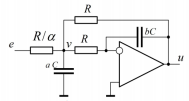
\includegraphics[width=0.3\linewidth]{pic12.png}
\end{figure}

$f_{max} = 4.980k$, $\Delta f = 338$ - ширина полосы по уровню 0.7.
$Q=\frac{f_{max}}{\Delta f} = 14.7$, $QK_0 = 73.5$ - пиковое усиление.

Построим график зависимости частоты пика от $R_2$

\begin{center}
\begin{tabular}{|c|c|c|c|c|c|c|c|c|}
\hline 
$R_2$ & 100 & 300 & 500 & 700 & 900 & 1100 & 1300 \\ 
\hline 
$f$ & 12,7k & 7,6k & 6,1k & 5,3k & 4,7k & 4,4k & 4,1k \\ 
\hline 
\end{tabular} 
\end{center}


\begin{figure}[h!]
    \centering
    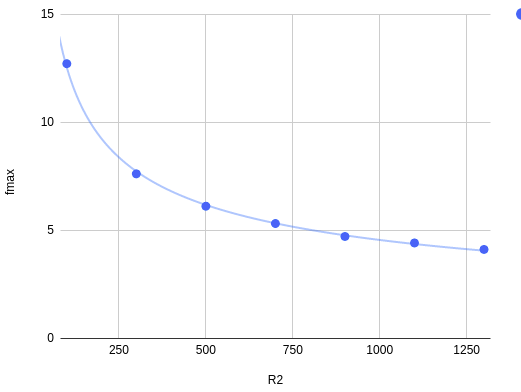
\includegraphics[width=0.6\linewidth]{pic14.png}
\end{figure}


На практике:


\begin{equation*}
	f_{max} = 5.05k, \hfill K_0 = 5.77
\end{equation*}




\end{document}